\subsection{Policies}
\label{subsec:policies}

Our policies (denoted by $\rho$) usually affect one of three contact types: education,
work and other contacts.
% households
Germany had no policies limiting contacts within households so there are no policies on
them in our model.\footnote{Household contacts can, however, be reduced when individuals
quarantine themselves after developing symptoms, for example. This happens to a lesser
degree than other contacts to capture difficulties in isolation within the home.}
% educ models
% educ policies

% summary
For nurseries, preschools and schools we implement vacations as announced by the German
federal states as well as school closures, emergency care and rotating schooling
schedules where only one half of students attends every other week or day. An
approximation of the share of contacts still taking place with the different school
regulations can be found in Figure~\ref{fig:school_multiplier}. Note that schooling
policies are decided on the state level and usually involved rules that depend on local
incidences. We simplify these rules to one federal policy from the federal incidence and
the policies of the three most populous federal states (North Rhine-Westphalia, Bavaria
and Baden-Württemberg).

% young educ
The policies for preschools and nurseries are similar to the school policies but simpler.
Until November children attend completely normally, starting in November with increased
hygiene measures. Nurseries and preschools stay open until mid December. From mid
December until January 10, nurseries and preschools were nearly completely closed. If
parents could credibly demonstrate that both parents work in systemically relevant
professions and no other child care arrangement was possible, nurseries and preschools
offered so called ``emergency care''. We assume 10\% of children qualified and used
emergency care during this time. After January 10 when more and more parents returned to
work the rules for emergency care were made less strict and we assume a third children
attended to nursery and preschool. This policy stayed in place until February 20.
Afterwards, preschools and nurseries opened normally until mid March. Then during the
third wave the restrictions February were put back into place until end of April when
nurseries and preschools opened again and stayed open \citep{KiTa_BY, KiTa_NRW, KiTa_BW,
KiTa_BWa, KiTa_BYa}.

% school

% work
For work contacts we use the reductions in work mobility reported by the Google Mobility
Data \citep{Google2021} to calibrate the reduction in physical work contacts
($\rho_{w,\:attend,\:t}$). Reductions in work contacts are not random but governed
through a work contact priority where the policy changes the threshold below which
workers stay home. Figure \ref{fig:work_multiplier} shows the share of workers that go to
work over time at the federal German level. We use the data on the state level to account
for local holidays and differences in state regulations.
% hygiene umltiplier
In addition, for both work and school contacts we assume that hygiene measures (such as
masks, ventilation and hand washing) became more strict and more conscientiously observed
in November, leading to a reduction of 33\% in the number of contacts with the potential
to transmit Covid-19 ($\rho_{hygiene}$).


\begin{figure}[ht]
    \centering
    \begin{subfigure}[b]{0.425\textwidth}
        \centering
        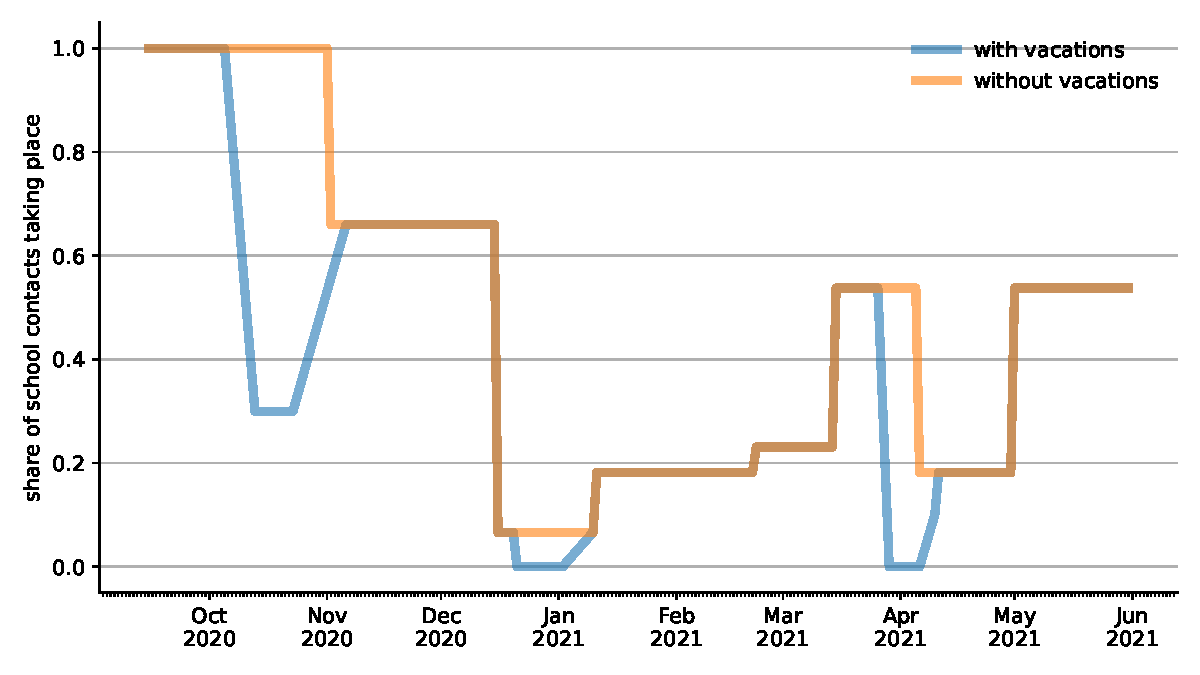
\includegraphics[width=\textwidth]{figures/results/figures/data/school_multiplier_comparison}
        \caption{{School Attendance}}
        \label{fig:school_multiplier}
    \end{subfigure}
    \hfill
    \begin{subfigure}[b]{0.425\textwidth}
        \centering
        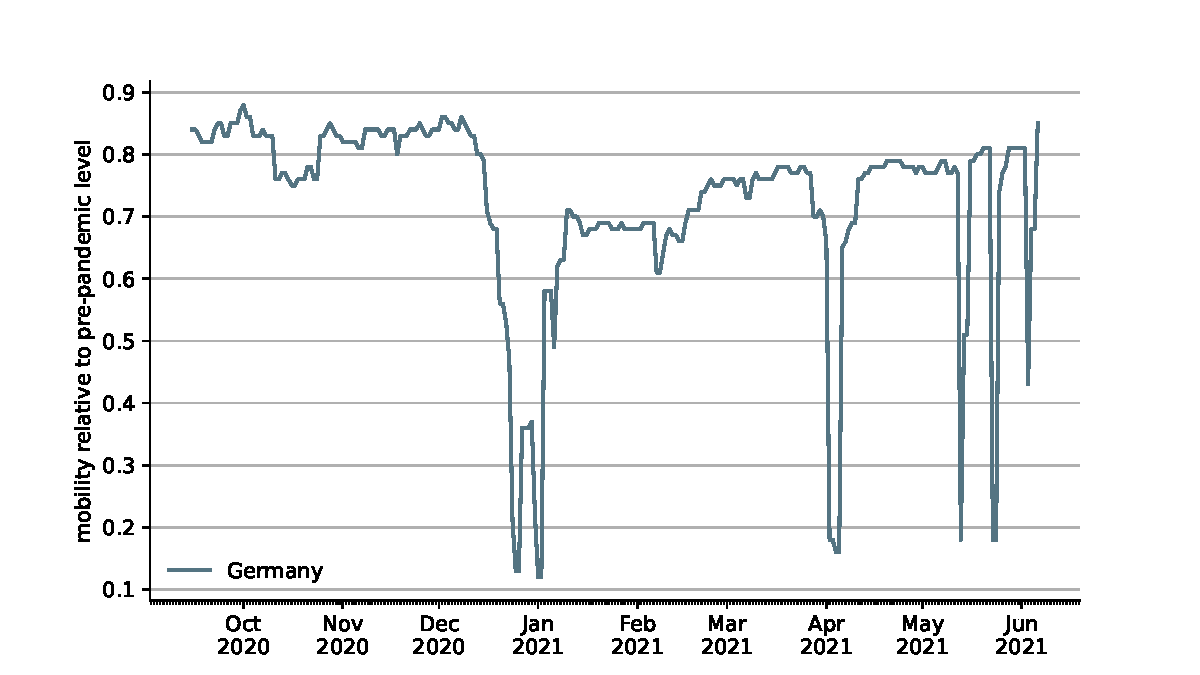
\includegraphics[width=\textwidth]{figures/results/figures/data/work_multiplier_since_sep}
        \caption{Work Attendance}
        \label{fig:work_multiplier}
    \end{subfigure}

    \vskip3ex

    \caption{The Contact Reduction Effects of School and Work Attendance Policies}

    \floatfoot{\noindent \textit{Note:} The left figure shows the approximate share of
    school contacts taking place with and without vacations factored in. The dates on
    which schools have vacation are decided at the state level. Vacations are directly
    implemented in our model with no school contacts taking place on weekends and during
    vacations (by federal state) just like the schooling mode (full operation, emergency
    care, rotating schemes with half class sizes etc.). The figure is, thus, only an
    illustration that shows the approximate share of contacts taking place compared to
    the pre-pandemic level with and without vacations. The difference between the lines
    show when vacations take place and to what degree. For example all states have fall
    vacations but the timing varies strongly between states while all states close
    schools during the Christmas holidays. The right figure shows the work mobility as
    reported by \cite{Google2021}. We take this as a proxy of the share of workers who
    still have physical work contacts ($\rho_{w,\:attend,\:t}$). The figure interpolates
    over weekends as we handle weekend effects through information on work on weekends in
    the German census data we use. The figure shows the share for Germany as a whole. To
    capture the effect that local policies, school vacations, etc. have on work contacts
    we use the data on the state level to determine which workers go to work depending on
    the state they live in.}
    \label{fig:multipliers}
\end{figure}

Lastly, for the other contacts category ($\rho_{other,\:t}$) we could not calibrate the
policies from data but estimated the policy effects. The estimation and values are
detailed in Section~\ref{subsec:estimated_params} and Figure~\ref{fig:other_multiplier}.

\FloatBarrier

